\documentclass[10pt,a4paper]{article}
\usepackage[T1]{fontenc}
\usepackage[utf8]{inputenc}
\usepackage{lmodern}
\usepackage[margin=2cm]{geometry}
\usepackage{amsmath,amssymb}
\usepackage{graphicx}
\usepackage{booktabs}
\usepackage{microtype}
\usepackage[font=small,labelfont={bf,color=teal},skip=3pt]{caption}
\usepackage[numbers,sort&compress]{natbib}
\usepackage{titlesec}
\usepackage{enumitem}
\usepackage{xcolor}
\usepackage[hidelinks]{hyperref}

\titlespacing*{\section}{0pt}{7pt}{3pt}
\titlespacing*{\subsection}{0pt}{5pt}{2pt}
\definecolor{teal}{HTML}{1f6f6b}
\definecolor{brick}{HTML}{b5452f}
\titleformat*{\section}{\large\bfseries\sffamily\color{teal}}
\titleformat*{\subsection}{\normalsize\bfseries\sffamily}
\setlength{\parskip}{2pt}
\setlength{\textfloatsep}{8pt}
\setlength{\floatsep}{6pt}
\setlength{\abovedisplayskip}{3pt}
\setlength{\belowdisplayskip}{3pt}
\setlist{nosep,leftmargin=1.2em}
\newcommand{\Hc}{\bar H}
\newcommand{\ndis}{n_{\mathrm{dis}}}

\begin{document}

%% ------------------------------------------------------------------ cover page
\begin{titlepage}
\centering
\vspace*{3.5cm}
{\LARGE\bfseries GAN on MNIST with a fixed generator:\\[4pt]
spectral normalization and rejection sampling\par}
\vspace{1.2cm}
{\large Nourcène Brahem, Lukas Tabouri, Manel Wafra --- DataLab A2, group CLM 34\par}
\vspace{0.5cm}
{\large 11 November 2026\par}
\vspace{1.5cm}
{\normalsize Master IASD \textperiodcentered{} Data Science Lab \textperiodcentered{} Assignment 2: train a GAN on MNIST with the provided generator architecture\par}
\vfill
\end{titlepage}
\setcounter{page}{1}

%% ------------------------------------------------------------------ 1
\begin{center}\textbf{Abstract}\end{center}
\vspace{-4pt}
{\small\leftskip=1.2em\rightskip=1.2em
With the provided MLP generator, the starter GAN collapses on one seed in three and otherwise reaches FID 44.5. We study one lever, the strength and smoothness of the discriminator. At training time, we cross spectral normalization (SN) with the number of discriminator steps per generator step, for the starter BCE loss and the hinge loss, at equal generator updates and over three seeds. Neither factor helps alone: five steps without SN collapse every seed onto a single digit, and SN with one step learns too slowly. Together they raise precision and recall at once (hinge: FID $42.0\to17.8$, precision $0.44\to0.65$, recall $0.46\to0.60$), whereas training an unconstrained discriminator longer leads to mode dropping. At inference, discriminator rejection sampling improves a weak generator (FID $42.0\to37.2$) but not a well-trained one, and its effect depends on how the density ratio is estimated. On the platform, our best submission reaches FID 14.4, precision 0.82 and recall 0.61.\par}
\vspace{2pt}

\section{Question and approach}
With the starter training, one run in three collapses within two epochs, and the runs that survive reach FID $44.5$ with precision $0.35$. Both failures point to the discriminator $D$: it can become so confident that the generator $G$ receives no useful gradient, or so sharp that $G$ settles on the few samples it accepts. We therefore study one lever, \emph{how strong and how smooth the discriminator is}, at training time and at inference time, with the generator architecture fixed:
\begin{itemize}
\item \textbf{Training.} Spectral normalization (SN) of $D$ \cite{miyato2018}, crossed with the number of $D$ updates per $G$ update, $\ndis\in\{1,5\}$, for two losses. \emph{H1: a Lipschitz-constrained $D$ can be trained harder without collapsing $G$, so precision and recall should rise together.}
\item \textbf{Inference.} Discriminator rejection sampling (DRS) \cite{azadi2019}, which uses $D$ to filter samples of a trained $G$. \emph{H2: rejection removes over-produced or poor samples, so precision should rise at constant recall, and more for a weak generator.}
\end{itemize}

%% ------------------------------------------------------------------ 2
\section{Setup, notation and protocol}
\textbf{Models and losses.} $G:\mathbb{R}^{100}\to[-1,1]^{784}$ is the provided MLP, unchanged in every run; $D:\mathbb{R}^{784}\to\mathbb{R}$ is the starter MLP and outputs a logit $D(x)$ ($\sigma$ is the sigmoid). We use the non-saturating BCE loss of the starter code and the hinge loss of \cite{miyato2018,lim2017}:
\begin{align*}
\text{BCE:}\quad & L_D=-\mathbb{E}\log\sigma(D(x))-\mathbb{E}\log(1-\sigma(D(G(z)))),\quad L_G=-\mathbb{E}\log\sigma(D(G(z))),\\
\text{hinge:}\quad & L_D=\mathbb{E}\max(0,1-D(x))+\mathbb{E}\max(0,1+D(G(z))),\quad L_G=-\mathbb{E}\,D(G(z)).
\end{align*}
SN replaces each weight matrix $W$ of $D$ by $W/\sigma_{\max}(W)$, with $\sigma_{\max}$ estimated by one power iteration per step; since leaky ReLU is 1-Lipschitz, $D$ becomes 1-Lipschitz. $\ndis$ is the number of $D$ steps per $G$ step.

\textbf{Tuning.} We compare configurations taken from the literature rather than searching hyperparameters for the best score. BCE runs keep the starter optimizer (Adam, lr $2\cdot10^{-4}$, $\beta=(0.9,0.999)$). Hinge runs use the setting of \cite{miyato2018} (lr $2\cdot10^{-4}$, $\beta=(0.5,0.999)$, their setting C), with $\ndis\in\{1,5\}$. Each cell of the ablation changes one factor; the only other knob we varied is the training length. The exact setting A of \cite{miyato2018} (lr $10^{-4}$, $\beta_2=0.9$, $\ndis=5$) failed for all six runs, with and without SN: every sample converges to the same blob within 50 epochs. We report this as a sensitivity result and leave these runs out of the analysis.

\textbf{Budget.} Every run gets the same number of generator updates, $93.8$k (100 epochs of 938 batches at $\ndis=1$, 500 epochs at $\ndis=5$), so a 5-step run costs about $3.5\times$ more time (Table~\ref{tab:ablation}). A control trains the hinge model with $\ndis=1$ for 500 epochs, i.e.\ the same number of $D$ updates as the 5-step runs. All configurations use three seeds (0, 1, 2), and we report mean (and standard deviation) over seeds.

\textbf{Metrics.} On 10\,000 samples: FID \cite{heusel2017} (Inception pool features), and precision/recall \cite{kynkaanniemi2019} (VGG-16 fc2 features, $k=5$). Precision is the fraction of samples inside the real manifold (quality), recall the fraction of real images inside the generated manifold (diversity). To read mode collapse directly, we also report $\Hc$, the entropy of the digit classes predicted by a pretrained MNIST classifier, divided by $\log 10$: $\Hc=1$ means balanced digits, $\Hc=0$ a single digit. It is a diagnostic only, never a selection criterion. Our FID matches the course platform within about one point on the models we submitted; the platform's precision and recall are higher in absolute value, so we compare models only within our evaluator.

\textbf{Pixel conversion.} The starter training normalises images to $[-1,1]$, but the starter \texttt{generate.py} saves $G$'s output clamped to $[0,1]$, which maps every grey level below the mid-point to black. We save $(x+1)/2$, the exact inverse of the training normalisation, for every model and metric. The generator is unchanged.

%% ------------------------------------------------------------------ 3
\section{Training: spectral normalization and the update ratio}



\begin{figure}[t]
\centering
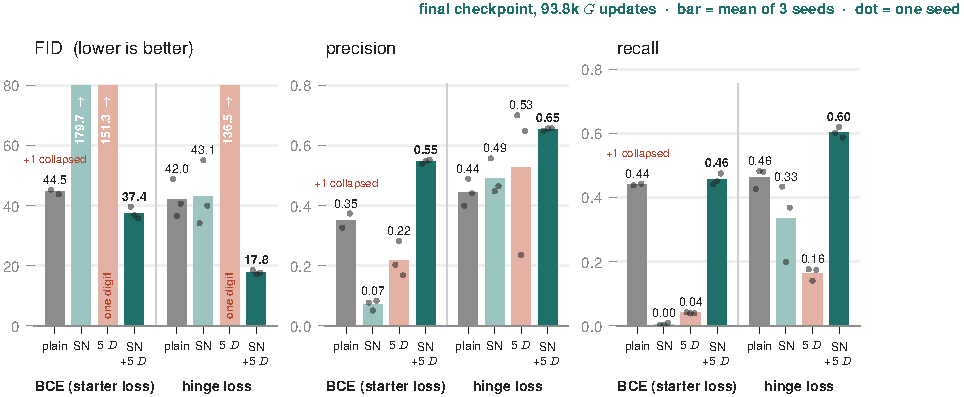
\includegraphics[width=\linewidth]{figs/fig_ablation.pdf}
\caption{The $2\times2$ ablation (SN $\times$ number of $D$ steps per $G$ step) for both losses, at equal generator updates. Bars cut at the top are written inside; ``one digit'': every seed ends on a single digit ($\Hc<0.3$).}
\label{fig:ablation}
\end{figure}

\begin{figure}[t]
\centering
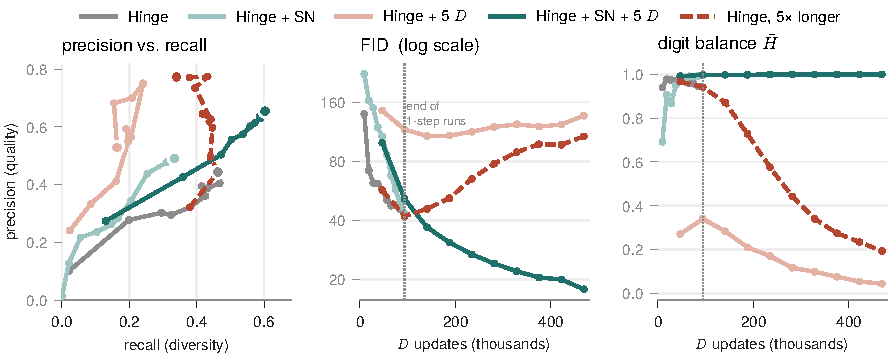
\includegraphics[width=\linewidth]{figs/fig_dynamics.pdf}
\caption{Training dynamics with the hinge loss, mean over seeds, one point per checkpoint (every $9.4$k generator updates). Left: trajectory in the precision--recall plane (large dot = final checkpoint; up = quality, right = diversity). Centre and right: FID and digit balance $\Hc$ against the number of $D$ updates; the 5-step runs and the $5\times$ longer run get the same number of $D$ updates.}
\label{fig:dynamics}
\end{figure}

\begin{figure}[t]
\centering
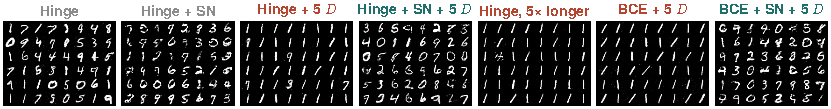
\includegraphics[width=\linewidth]{figs/fig_grids.pdf}
\caption{Samples at the final checkpoint: first 48 of the 64 fixed latent vectors used for every run (same $z$ in every panel, not selected). Red: runs ending on one digit; teal: SN with five steps.}
\label{fig:grids}
\end{figure}

\textbf{The two factors only help together, and with both losses.} Fig.~\ref{fig:ablation} and Table~\ref{tab:ablation} show the same structure for BCE and hinge. Five $D$ steps without SN collapse every seed onto a single digit ($\Hc=0.00$ for BCE, $0.04$ for hinge; Fig.~\ref{fig:grids}). SN with one step does not help either: with BCE it barely learns (precision $0.07$), and with hinge it keeps FID unchanged while recall drops from $0.46$ to $0.33$. Only SN with five steps improves the three metrics at once, on every seed and for both losses: with hinge, FID goes from $42.0$ to $17.8$, precision from $0.44$ to $0.65$ and recall from $0.46$ to $0.60$. The seed spread also shrinks (FID standard deviation $6.2\to0.7$). The intervention does not trade quality for diversity: in Fig.~\ref{fig:dynamics} (left) the SN, 5-step trajectory is the only one that keeps moving up \emph{and} right until the end.

\textbf{Stronger unconstrained discriminators lead to mode dropping.} We gave an unconstrained $D$ more training in two independent ways: five steps per $G$ step, and five times more epochs at one step (the same number of $D$ updates). Both end with almost a single digit on every seed: $\Hc=0.04$ and $0.19$ for hinge, $0.00$ for BCE with five steps (Fig.~\ref{fig:dynamics}, right). The precision--recall trajectories show how this happens. With five steps, or with longer training (Fig.~\ref{fig:dynamics}, left), precision keeps rising (up to $0.77$) while recall stalls or falls: the samples become sharper but less varied, and the grids end with almost only ``1''s, the simplest digit. The long run loses digits gradually rather than suddenly ($\Hc$: $0.94\to0.19$ between 100 and 500 epochs), which points to a drift and not to a numerical failure. FID detects it, since it rises from $42$ to $107$ after the best checkpoint of the long run (Fig.~\ref{fig:dynamics}, centre). Precision alone would rank the collapsed model best. Our interpretation, consistent with these measurements, is that an unconstrained $D$ trained close to optimality becomes sharp around the real data, and its gradient pushes $G$ towards the few regions it scores highest.

\textbf{SN makes the discriminator slower, and more steps compensate.} With SN and one step, $D$ falls behind: BCE + SN reaches only FID $180$, and hinge + SN is still improving at the end of the budget (FID $48.8\to43.1$ over the last 10 epochs; Fig.~\ref{fig:dynamics}). Five steps move BCE + SN from FID $180$ to $37$, and hinge + SN from $43$ to $18$. So the same knob, more discriminator training per $G$ step, has opposite effects depending on the constraint. It hurts an unconstrained $D$ and helps a Lipschitz one. This is the behaviour H1 predicts, and the reasoning behind training a Lipschitz critic close to optimality in WGANs \cite{arjovsky2017}.

\begin{table}[ht]
\centering\small
\setlength{\tabcolsep}{4.5pt}
\begin{tabular}{llcrccccr}
\toprule
Loss & $D$ schedule (per $G$ step) & SN & FID $\downarrow$ & Precision $\uparrow$ & Recall $\uparrow$ & $\Hc$ & 1-digit & min \\
\midrule
BCE   & 1 step (starter)           & --         & $44.5\pm1.1^{*}$ & 0.35 & 0.44 & 0.97 & 1/3 & 8 \\
      & 1 step                     & \checkmark & $179.7\pm3.3$ & 0.07 & $<$0.01 & 0.87 & 0/3 & 16 \\
      & 5 steps                    & --         & $151.3\pm8.3$ & 0.22 & 0.04 & 0.00 & 3/3 & 29 \\
      & 5 steps                    & \checkmark & $\mathbf{37.4\pm2.0}$ & \textbf{0.55} & \textbf{0.46} & 1.00 & 0/3 & 57 \\
\midrule
Hinge & 1 step                     & --         & $42.0\pm6.2$ & 0.44 & 0.46 & 0.94 & 0/3 & 9 \\
      & 1 step                     & \checkmark & $43.1\pm10.8$ & 0.49 & 0.33 & 1.00 & 0/3 & 16 \\
      & 5 steps                    & --         & $136.5\pm18.6$ & 0.53 & 0.16 & 0.04 & 3/3 & 28 \\
      & 5 steps                    & \checkmark & $\mathbf{17.8\pm0.7}$ & \textbf{0.65} & \textbf{0.60} & 1.00 & 0/3 & 57 \\
      & 1 step, $5\times$ epochs & -- & $107.1\pm5.1$ & 0.77 & 0.34 & 0.19 & 3/3 & 40 \\
\bottomrule
\end{tabular}
\caption{Final checkpoint, mean over three seeds ($\pm$ standard deviation for FID). All runs have $93.8$k generator updates, except the last row ($5\times$ more). $\Hc$: normalised entropy of the predicted digit classes. 1-digit: seeds with $\Hc<0.3$. $^{*}$Mean of the two seeds that train; the third collapses after two epochs (FID 374).}
\label{tab:ablation}
\end{table}

\textbf{More compute alone does not explain the gain.} At equal numbers of $D$ updates, the 1-step hinge model trained $5\times$ longer ends at FID $107$, against $17.8$ for SN with five steps (Fig.~\ref{fig:dynamics}). Its best checkpoint ($42.0$) comes after 100 epochs. The 57 minutes of the SN, 5-step runs (vs.\ 9) buy a better model only because the constraint lets $D$ use them.

\textbf{Loss.} At SN with five steps, hinge reaches FID $17.8$ against $37.4$ for BCE, with higher precision and recall. Our hinge runs also use $\beta_1=0.5$ instead of $0.9$, so this gap measures the hinge setting of \cite{miyato2018} as a whole, loss and optimizer together.

%% ------------------------------------------------------------------ 4
\section{Inference: discriminator rejection sampling}
\textbf{Method.} At the optimum of the BCE loss, $D(x)=\log\frac{p_{\text{data}}(x)}{p_G(x)}$, so $r(x)=e^{D(x)}$ estimates the density ratio. DRS \cite{azadi2019} accepts a sample with probability $a(x)=\big(1+e^{\gamma}(M/r(x)-1)\big)^{-1}$, where $M=\max r$ is estimated on 10\,000 calibration samples, and $\gamma$ is set so that the mean acceptance on these samples is $1/K$. A budget $K$ thus costs $K$ generator passes per kept image. Since the method assumes an optimal discriminator, we compare three estimators of $r$: the \emph{final} $D$ of GAN training; the same $D$ \emph{fine-tuned} for 3 epochs with BCE against the frozen $G$ (as in \cite{azadi2019}); and a $D$ \emph{trained from scratch} against the frozen $G$ (starter architecture, no SN, BCE, early stopping on held-out real digits and fresh samples). The last estimator is independent of GAN training. It reaches 98.5–99.2\% held-out accuracy on the weak generators and 96.4–97.6\% on the best one. Fig.~\ref{fig:drs} compares the three estimators at $K=5$ and shows the change in FID for $K\in\{1,2,5,10\}$, on a weak generator (hinge) and on our best one (hinge, SN, 5 steps).

\begin{figure}[t]
\centering
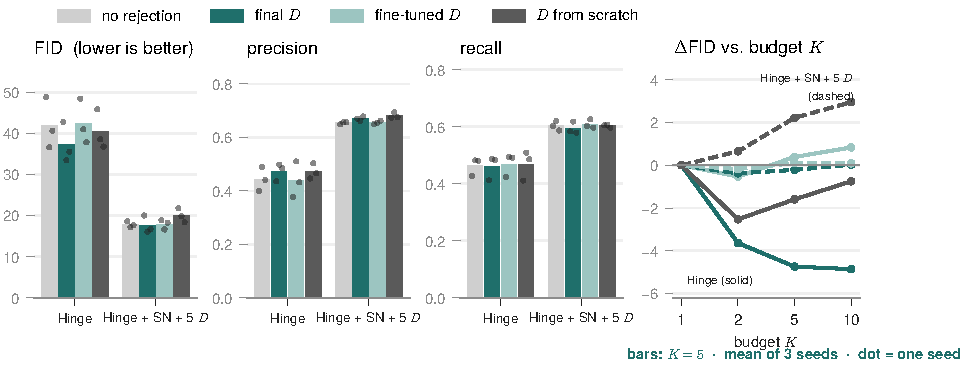
\includegraphics[width=\linewidth]{figs/fig_drs.pdf}
\caption{DRS with three estimators of the density ratio. Bars: FID, precision and recall at $K=5$ (acceptance $1/5$), for a weak and a strong generator. Right: change in FID relative to plain sampling as the budget $K$ grows (solid: hinge; dashed: hinge + SN + 5 $D$).}
\label{fig:drs}
\end{figure}

\textbf{Results.} On the weak generator, DRS with the final $D$ lowers FID from $42.0$ to $37.2$ at $K=5$, with precision $+0.03$ and recall unchanged (within $\pm0.01$, below the seed spread). The gain saturates: $38.4$, $37.2$ and $37.1$ for $K=2,5,10$, so most of it costs only a factor of two. The same holds for the starter BCE generator (FID $44.5\to37.6$). On our best generator, the final $D$ changes FID by less than $0.5$. There is little left to correct, since the training intervention already removed what DRS removes. The fine-tuned $D$ brings nothing on either generator.

The $D$ trained from scratch behaves as H2 predicts on precision ($+0.03$ on both generators, up to $0.68$ on the best one) and keeps recall. Its FID, however, gets \emph{worse} as $K$ grows on the best generator ($17.8\to20.8$ at $K=10$), and $\Hc$ falls from $0.999$ to $0.968$: rejection becomes digit-selective. This D is a near-perfect classifier, so its log-ratio is extreme and driven by a few features. Rejection then shifts the class proportions: FID is sensitive to this, while precision and recall, which only check each sample against the real manifold, are not. So the most accurate classifier is not the best ratio estimator for DRS, and the estimator matters as much as the budget. The fact that the final hinge $D$, which is not a log-ratio estimator in theory, works best on the weak generator suggests that its value comes from being trained against that generator's own artefacts (a hypothesis).

\textbf{Comparison with latent truncation.} Resampling latent coordinates with $|z_i|>\psi$ \cite{brock2019} lowers FID on the best generator at $\psi=1.5$ ($15.4$), but it reduces precision ($0.62$) and recall ($0.54$). It gets worse for smaller $\psi$ ($\psi=1$: FID $18.8$, P $0.51$, R $0.41$). Here FID and precision/recall disagree. Truncation moves samples towards the mode of the latent prior, and on MNIST, unlike on natural images, this does not raise precision.

%% ------------------------------------------------------------------ 5
\section{What the experiments support}
\textbf{Supported (3 seeds, controlled comparisons).} (i) Constraining $D$ with SN and training it with five steps per $G$ step improves quality and diversity together, with both losses. Neither factor alone does, and longer training of an unconstrained $D$ degrades the model. (ii) Strengthening an unconstrained $D$, by more steps or more epochs, ends in mode dropping, visible as rising precision with falling recall and $\Hc$. (iii) DRS improves a weak generator, saturates quickly in $K$, and adds almost nothing to a well-trained one. Its outcome depends on the ratio estimator.

\textbf{Scope and open questions.} The study compares one and five $D$ steps per $G$ step; how the gain evolves between and beyond these two values is a natural extension of this design. At the shared budget of $93.8$k generator updates, hinge + SN with one step is still improving, so the comparison measures the gain at equal generator updates rather than at convergence. Our hinge runs follow the optimizer setting of \cite{miyato2018} ($\beta_1=0.5$), which the comparison with BCE keeps attached to the loss. The conclusions hold for this optimizer setting; setting A (lr $10^{-4}$, $\beta_2=0.9$) did not train with or without SN, which indicates that the method is sensitive to the optimizer. The mechanisms proposed above, a sharp unconstrained $D$ and a narrow logit range limiting DRS on an SN discriminator, are consistent with all our measurements; gradient norms and logit ranges would test them directly.

\textbf{Leaderboard.} With the generator trained with SN and five steps (seed 1, pixels saved as $(x+1)/2$), truncation at $\psi=1.5$ obtained FID $14.4$, precision $0.82$ and recall $0.61$ on the platform. DRS with the final $D$ at $K=5$ obtained FID $16.5$, precision $0.76$ and recall $0.66$, the best recall of our submissions, in 78\,s on CPU. The starter baseline got $30.6$, $0.52$ and $0.22$.

\begingroup
\small
\setlength{\bibsep}{1pt}
\begin{thebibliography}{9}
\bibitem{miyato2018} T.~Miyato, T.~Kataoka, M.~Koyama, Y.~Yoshida. Spectral normalization for generative adversarial networks. ICLR 2018.
\bibitem{lim2017} J.~H.~Lim, J.~C.~Ye. Geometric GAN. arXiv:1705.02894, 2017.
\bibitem{azadi2019} S.~Azadi, C.~Olsson, T.~Darrell, I.~Goodfellow, A.~Odena. Discriminator rejection sampling. ICLR 2019.
\bibitem{kynkaanniemi2019} T.~Kynkäänniemi, T.~Karras, S.~Laine, J.~Lehtinen, T.~Aila. Improved precision and recall metric for assessing generative models. NeurIPS 2019.
\bibitem{heusel2017} M.~Heusel, H.~Ramsauer, T.~Unterthiner, B.~Nessler, S.~Hochreiter. GANs trained by a two time-scale update rule converge to a local Nash equilibrium. NeurIPS 2017.
\bibitem{arjovsky2017} M.~Arjovsky, S.~Chintala, L.~Bottou. Wasserstein generative adversarial networks. ICML 2017.
\bibitem{brock2019} A.~Brock, J.~Donahue, K.~Simonyan. Large scale GAN training for high fidelity natural image synthesis. ICLR 2019.
\end{thebibliography}
\endgroup

\end{document}
